%======================================================================
\section{Setup}\label{sec:setup}
%======================================================================
All models are trained on the clean split with the main report's architecture and hyper-parameters
($H=128$, $d=10$, $\lambda_J=10^{-3}$, same seed and batches), and early stopping with a patience of
$150$ epochs; the only differences between runs are the field terms. Fields carry an $L_2$ penalty
$10^{-4}\|W\|^2$.
\begin{description}[leftmargin=1.2em,itemsep=1pt]
\item[Baseline] field-free AttentionDCA (best epoch \EpBase, validation NLPL \ValBase).
\item[M2] $+$ per-site fields $h_i(a)$, learned jointly (\ValMtwo).
\item[C1] the baseline plus the restraint \eqref{eq:dJdh} at sampling time; nothing is retrained.
      $\lambda\in\{0.25,1,4,16,64\}$.
\item[C3] fields $h_i(a\mid\bm z)=\sum_fW_f(i,a)\phi_f(\bm u)$, $\phi=(1,u_1,u_2,u_1^2,u_2^2,u_1u_2)$,
      $\bm u$ the standardised coordinates, trained on $(\bm x,\PC(\bm x)+\sigma\bm\epsilon)$ with fresh
      noise at every batch, for $\sigma=1,\,0.5,\,0.25$ (validation NLPL \ValCthreeOne, \ValCthree,
      \ValCthreeQ, scored with the noiseless coordinate). At sampling time $\bm z=\bm t$; a gain
      $\kappa$ optionally multiplies the $\bm z$-dependent part of the field.
\end{description}
\textbf{Targets} are the three k-means centres of the main report (C0 = the under-sampled HscB-like
cluster, C1, C2). For each method, target and setting, $3000$ chains start from random
\emph{training} sequences --- mostly in another cluster, so they have to travel --- and run $500$
sweeps. The restrained chains converge within $50$ sweeps for $\lambda\ge4$ and $\sim100$ for
$\lambda=1$ (figure in the appendix). The PCA frame is the one used in every figure of the main
report (fitted on the test set); it is a fixed linear map, $V$ and $\bm m$ are just constants.

\textbf{Metrics}, all against the natural \emph{test} sequences of the target cluster
(\NatNA, \NatNB, \NatNC\ sequences for C0, C1, C2; reweighted):
distance $\|\PC-\bm t\|$; \emph{overshoot}, the signed miss along the line from the family centre to
the target ($>0$: beyond the target, $<0$: stopped short); share landing in the target cluster;
$r(f_i)$ and $r(C_{ij})$; HPD motif retained (columns 28--30, present in $\ge99\%$ of natural
sequences); mean energy under one common judge (the baseline model, so C1 and C3 are on the same
scale; natural cluster means \NatEA, \NatEB, \NatEC); mean distance to the closest training
sequence ($d_\text{train}$, novelty) and mean pairwise distance within the pool (div., diversity).
Because $C_{ij}$ estimates are noisy, \emph{every} pool is evaluated at the same size, $3000$; the
natural ceiling is a weight-proportional draw of $3000$ training sequences of the cluster. With
these sizes the ceiling is $r(C_{ij})=\CeilA$, \CeilB, \CeilC\ --- lower than the full-family
values of the main report simply because a cluster has fewer sequences.

%======================================================================
\section{M2: explicit fields}\label{sec:m2}
%======================================================================
\begin{table}[h]\centering\small
\begin{tabular}{lcccccc}
\toprule
 & val.\ NLPL & test NLPL & $r(f_i)$ & $r(C_{ij})$ / slope & shares C0/C1/C2 (\%) & $\Delta F_{C0}$ \\
\midrule
natural & -- & -- & -- & -- & 14/39/47 & -- \\
no fields & 81.97 & 78.57 & 0.930 & 0.744 / 0.28 & 5/86/9 & 1.04 \\
M2 (+ fields) & 82.03 & 78.49 & 0.938 & 0.791 / 0.34 & 5/83/12 & 1.12 \\
\bottomrule
\end{tabular}

\caption{Fields versus no fields, same training protocol. NLPL in nats per sequence; $r$ and slope of
the generated statistics against the natural test set (full family); shares by nearest cluster
centre; $\Delta F_{C0}=-\ln(s^\text{gen}_{C0}/s^\text{nat}_{C0})$.}
\label{tab:m2}
\end{table}

\paragraph{Fields are learned, but they replace couplings rather than add information.} The fields
are far from zero (mean $|h_i(a)|=\FieldAbs$) and the coupling norm drops from \JfrobBase\ to
\JfrobMtwo, yet the pseudo-likelihood is unchanged (Table~\ref{tab:m2}: validation \ValBase\ vs
\ValMtwo, test \NLPLtestBase\ vs \NLPLtestMtwo). This confirms the premise of AttentionDCA: the
conserved-residue and gap columns of the value matrices $V^h$ already act as fields. The generated
statistics improve modestly ($r(f_i)$ \rfBase$\to$\rfMtwo, $r(C_{ij})$ \rCBase$\to$\rCMtwo), so fields
are a cheap, harmless addition.

\paragraph{Fields do not fix the missing cluster.} C0 receives $5\%$ of the samples with and without
fields ($\Delta F_{C0}=\dFzeroBase\to\dFzeroMtwo$). Figure~\ref{fig:m2} (right) shows why, using the
decomposition $F=\langle E\rangle-S$ of \S\ref{sec:sp}. In both models C0 lies about $20$ energy units
above C1 and $17$--$20$ nats higher in entropy; the two nearly cancel and leave a free-energy
difference of $2.8$--$2.9$ nats. A field shifts the energy of every sequence carrying a given
residue; it cannot, by itself, rebalance two basins whose weights are set by a near-cancellation
between energy and entropy. That balance is not what pseudo-likelihood measures --- it fits each
site's conditional given the rest of the sequence, never the relative mass of whole basins.

\begin{figure}[t]\centering
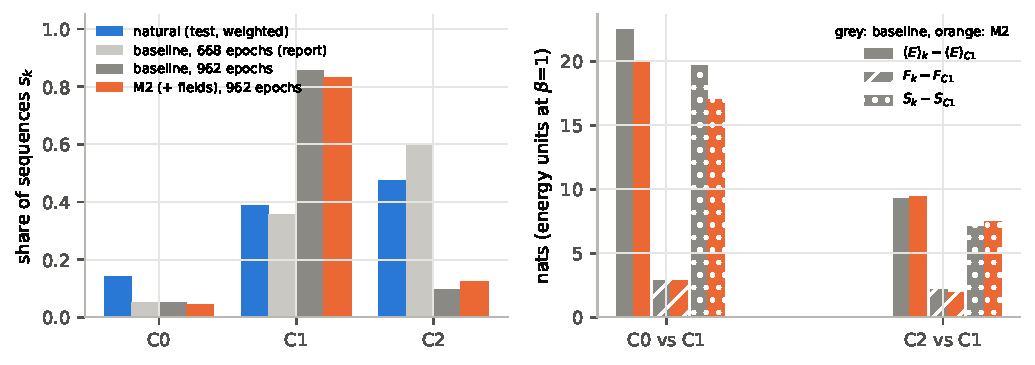
\includegraphics[width=0.92\textwidth]{m2_shares.pdf}
\caption{Left: cluster shares. The two grey bars (light, dark) are the \emph{same} field-free model at two
training lengths. Right: per-cluster mean energy, free energy and entropy of each model's own
samples, relative to C1 ($F_k=-\ln s_k$, $S_k=\langle E\rangle_k-F_k$, $\beta=1$).}
\label{fig:m2}
\end{figure}

\paragraph{A finding worth more than M2 itself: the mode weights depend on when training stops.}
The main report's model stopped at epoch \EpClean\ (patience 50); retraining it with the current code
reproduces its couplings bit for bit. The same run continued to epoch \EpBase\ (patience 150) has a
\emph{better} validation pseudo-likelihood (\ValClean$\to$\ValBase, $0.2$ nats per sequence) and
the same C0 deficit, but its C1/C2 balance has flipped: shares C0/C1/C2 go from \ShareClean\ to
\ShareBasep\ (natural \ShareNat). That is a $2.7$-nat swing in the relative free energy of C1 and C2
for $0.2$ nats of pseudo-likelihood --- and it makes the longer-trained model a \emph{worse}
generator of the family ($r(C_{ij})=\rCBase$, slope \sCBase, against $0.87$ for the report's model),
because full-family correlations are dominated by the contrast between clusters. Two consequences:
(i) the main report's statement that C1 and C2 are ``covered'' is true of that checkpoint but is not
a robust property of the method; the C0 deficit, by contrast, is present in every model trained;
(ii) the validation pseudo-likelihood cannot select a model for its sampling behaviour. Fixing the
mode weights needs an objective that sees them (M4, likelihood/PCD fine-tuning) or, as below, an
explicit choice of where to sample.

%======================================================================
\section{C1: the analytic restraint}\label{sec:c1}
%======================================================================
\begin{figure}[t]\centering
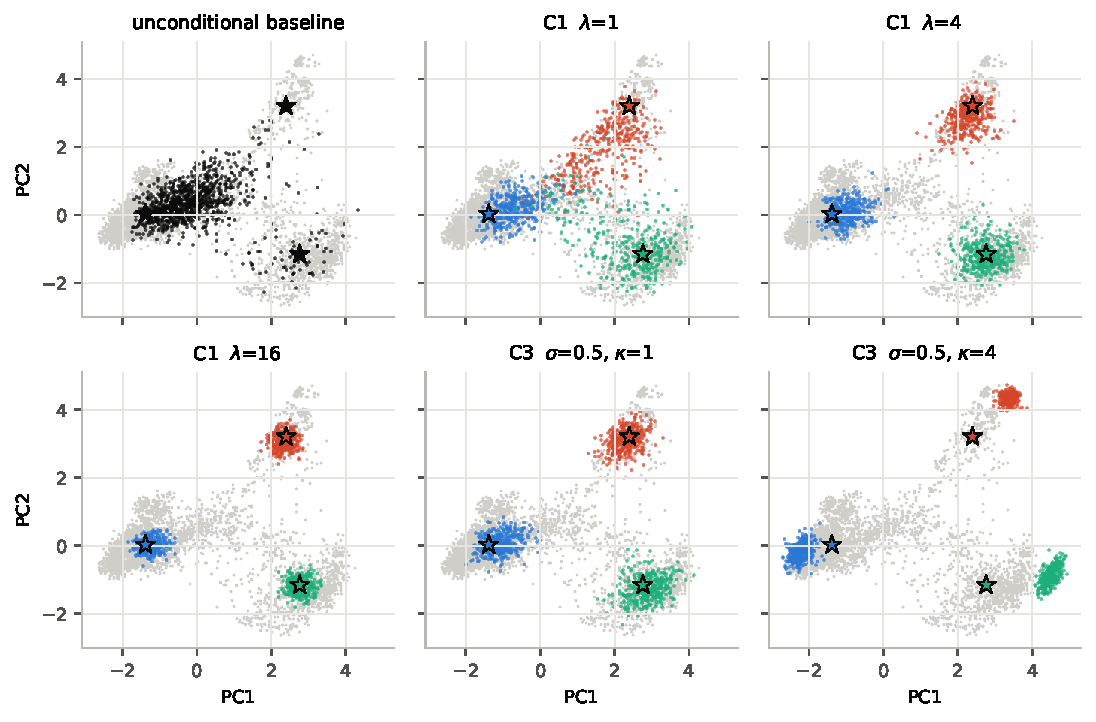
\includegraphics[width=0.86\textwidth]{cond_pca.pdf}
\caption{Samples in the PCA plane (grey: natural test). Stars: targets C0 (red), C1 (blue), C2
(green); points are coloured by the target they were aimed at. Top left: the unconditional baseline,
which visits C1 almost exclusively. Bottom right: C3 with its target field amplified by $\kappa=4$ ---
every pool lands \emph{beyond} its target.}
\label{fig:pca}
\end{figure}

\begin{figure}[t]\centering
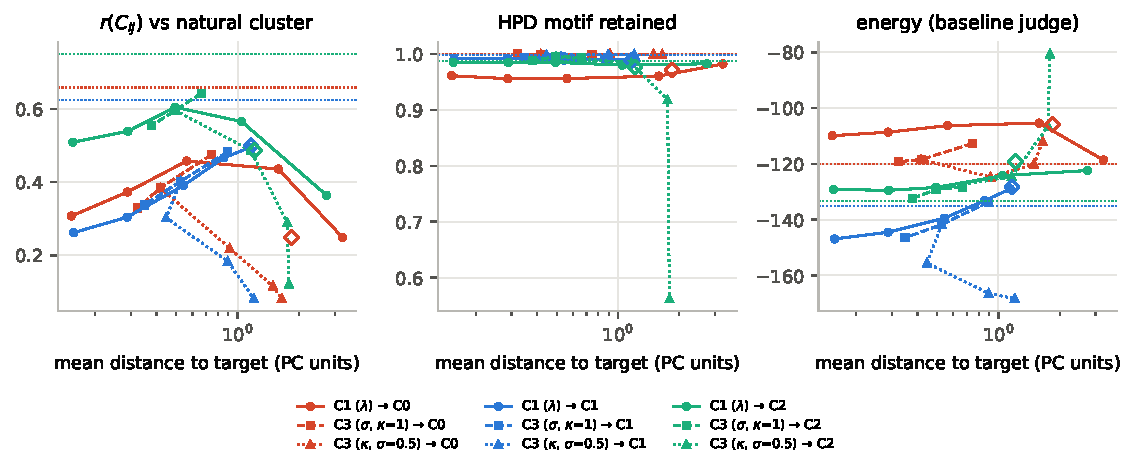
\includegraphics[width=\textwidth]{cond_tradeoff.pdf}
\caption{Accuracy--quality trade-off, one curve per method and target (colour). Solid circles: C1,
$\lambda=0.25\to64$ (right to left). Dashed squares: C3 at $\kappa=1$, $\sigma=1\to0.25$. Dotted
triangles: C3, $\sigma=0.5$, $\kappa=1\to8$. Open diamonds: rejection from the unconditional
baseline. Dotted horizontal lines: natural ceiling ($r(C_{ij})$) and natural cluster value (HPD,
energy).}
\label{fig:trade}
\end{figure}

\paragraph{It steers, to any target, including the one the model neglects.} Without restraint,
$5\%$, $86\%$ and $10\%$ of the chains end in C0, C1, C2. From $\lambda=4$ on, $100\%$ end in the
cluster they are aimed at (Figure~\ref{fig:pca}), and the mean distance to the target falls as
$1/\sqrt\lambda$ --- $0.5$, $0.3$, $0.15$ at $\lambda=4,16,64$, the width of the Gaussian window
of \S\ref{sec:pca}, Step~5. The response is monotone in $\lambda$, unlike $\beta_\mathrm{PCA}$ in the
previous study.

\paragraph{It keeps the protein.} The HPD motif is retained in $96$--$99\%$ of the samples at every
$\lambda$ (Tables~\ref{tab:C0}--\ref{tab:C2}), against $99$--$100\%$ for the natural clusters;
$r(f_i)$ against the target cluster's natural sequences is $0.96$--$0.99$ for $\lambda\ge1$.
The covariation agreement $r(C_{ij})$ \emph{peaks} at a moderate stiffness --- \ConeALfourrC\ for C0
and $0.605$ for C2 at $\lambda=4$, $0.49$ for C1 at $\lambda=0.25$ --- against ceilings \CeilA,
\CeilB, \CeilC, and declines for larger $\lambda$. Most of that decline is not damage but a mismatch
of scale: a natural cluster has a radius of about one PC unit, so a window of width $0.15$ samples
the \emph{centre} of the cluster rather than the cluster, and the pool loses the cluster's internal
variation (diversity drops from $0.56$ to $0.47$ for C1). \textbf{The useful regime is
$\lambda\approx1$--$4$}, a window comparable to the size of the region one wants.

\paragraph{Against rejection, the exact conditional.} Keeping only the unconditional samples that
fall in C0 gives $496$ sequences out of $10\,000$; at the same cost C1 produces $10\,000$. Where the
two can be compared they agree on what the model believes: C1 at $\lambda=4$ and rejection give C0
sequences of the same energy (\ConeALfourE\ vs $-106.0$), as they should if C1 samples the model's
own conditional. That energy is $14$ units above the natural C0 sequences (\NatEA): the model's C0
basin is not only under-weighted (\S\ref{sec:m2}) but also displaced towards higher energy, and C1,
which only restrains the coordinates, inherits it faithfully.

\paragraph{It inherits the prior's error at weak restraint.} The overshoot column is negative at
small $\lambda$: chains stop short of the target, on the side of the family centre ($-1.42$ for C0
at $\lambda=1$, where only $80\%$ reach the cluster). The restraint has to overcome the model's own
free-energy penalty on C0, so the weaker it is, the more the model's mis-weighting shows through.

%======================================================================
\section{C3: the learned conditional field}\label{sec:c3}
%======================================================================
\paragraph{At its natural setting it matches C1.} Knowing the coordinate improves the conditional
pseudo-likelihood by $0.4$, $0.9$ and $2.0$ nats for $\sigma=1,\,0.5,\,0.25$: the sharper the
coordinate, the more it says about each site. Sampled at $\bm z=\bm t$ with $\kappa=1$, C3 lands on
target with the accuracy of C1 at the matching $\lambda=1/\sigma^2$ (dashed vs solid curves of
Figure~\ref{fig:trade}; distances \CthreeAsHKonedist, $0.53$, $0.49$ at $\sigma=0.5$ against $0.56$,
$0.54$, $0.49$ for C1 at $\lambda=4$) and with comparable quality (HPD $99$--$100\%$,
$r(C_{ij})$ within $0.07$ of C1 for every target). This is the prediction of \S\ref{sec:pca}, Step 7: C3,
trained on noisy coordinates, learns the same distribution that C1 writes down.

\paragraph{Where it is better: the neglected cluster.} The one systematic difference is C0. C3 gets
closer to it at weak conditioning ($\sigma=1$: distance $0.74$, overshoot $-0.56$, against $1.59$
and $-1.42$ for C1 at $\lambda=1$), and its C0 sequences have lower energy (\CthreeAsHKoneE\ at
$\sigma=0.5$ against \ConeALfourE), closer to the natural C0 (\NatEA). The reason is the prior. C1
multiplies the \emph{unconditional} model, with its C0 free-energy error, by a window; C3 was trained
on (sequence, coordinate) pairs and learned the conditional directly from data, so it does not
inherit that error. This is the one place where a learned conditional earns its extra parameters
for a sequence-derived label.

\paragraph{Amplifying the target field reproduces the old failure, exactly as predicted.} With the
gain $\kappa$ on the $\bm z$-dependent field the samples \emph{overshoot}: $+0.84$, $+1.36$,
$+1.47$ for C0 and $+0.28$, $+0.84$, $+1.17$ for C1 at $\kappa=2,4,8$ (Figure~\ref{fig:pca}, bottom
right). Everything else degrades with it: diversity collapses to $0.16$ (C0) and $0.21$ (C1) ---
near-copies of one sequence --- $r(C_{ij})$ falls to $0.08$--$0.12$, and for C2 the HPD motif is lost
in $44\%$ of the samples while the energy rises to $-81$, $50$ units above the natural cluster. The
mechanism is the one derived in Step 7: $\kappa$ amplifies the field that pushes towards the target
but not the coupling term that holds the coordinate \emph{at} the target. This is the
$\beta_\mathrm{PCA}$ pathology of the previous study --- ``shifts too far right, loses the HPD
motif'' --- now reproduced on demand and explained.

%======================================================================
\section{Summary}\label{sec:sum}
%======================================================================
\begin{itemize}[leftmargin=*,itemsep=2pt]
\item \textbf{C1 works and needs no training.} Monotone control by $\lambda$, all three clusters
      reachable (C0 from $5\%$ to $100\%$), HPD kept, best covariation agreement at
      $\lambda\approx1$--$4$. It samples the model's own conditional, so it inherits the model's
      errors about a region (C0 is reached, but at too high an energy).
\item \textbf{C3 matches C1 at $\lambda=1/\sigma^2$} and is better on the neglected cluster because
      it learns the conditional from data instead of reweighting a biased prior. Use it at $\kappa=1$;
      amplifying it reproduces the old over-steering pathology.
\item \textbf{M2} leaves the pseudo-likelihood unchanged, slightly improves the generated
      statistics, and does not fix the mode weights.
\item \textbf{Mode weights are fragile under pseudo-likelihood}: $294$ more epochs moved the C1/C2
      balance by $2.7$ nats for a $0.2$-nat gain in validation PL, while C0 stayed at $5\%$ in every
      model.
\end{itemize}

\noindent\textbf{Next step suggested by these results.} Conditioning gives a direct, cheap fix for
the mode weights: draw a target $\bm t$ from the natural distribution of coordinates (the reweighted
training PCA points), then sample $\bm x\sim p(\bm x\mid\bm t)$ with C3 at $\kappa=1$ (or C1 at
$\lambda\approx4$). This is ancestral sampling of $p(\bm t)\,p(\bm x\mid\bm t)$: the cluster shares
are the natural ones \emph{by construction}, and the within-cluster statistics are those measured
here. It would remove both the C0 deficit and the training-length dependence of the C1/C2 balance
without retraining anything but C3.

\appendix
\section{Per-target tables and convergence}
\noindent Columns: mean distance to target; overshoot (signed, $>0$ beyond the target); \% landing in
the target cluster; $r(f_i)$, $r(C_{ij})$ against the natural test sequences of the cluster; \% with
the HPD motif; mean energy under the baseline judge; mean distance to the closest training
sequence; mean pairwise distance in the pool. All pools of size $3000$ except the rejection pool.

\begin{table}[h]\centering\scriptsize\setlength{\tabcolsep}{4pt}
\begin{tabular}{lccccccccc}
\toprule
 & dist. & overshoot & in $C_k$ (\%) & $r(f_i)$ & $r(C_{ij})$ & HPD (\%) & $E$ & $d_\text{train}$ & div. \\
\midrule
natural (train, ceiling) & 0.99 & -0.75 & 100 & 0.994 & 0.659 & 100 & -123.3 & 0.00 & 0.67 \\
rejection from baseline (n=496) & 1.84 & -1.70 & 100 & 0.928 & 0.248 & 97 & -106.0 & 0.49 & 0.69 \\
unconditional baseline & 3.89 & -3.47 & 5 & 0.684 & 0.158 & 99 & -126.3 & 0.39 & 0.62 \\
\midrule
C1 $\lambda{=}1$ & 1.59 & -1.42 & 80 & 0.963 & 0.436 & 96 & -105.4 & 0.48 & 0.70 \\
C1 $\lambda{=}4$ & 0.56 & -0.41 & 100 & 0.982 & 0.458 & 96 & -106.3 & 0.46 & 0.64 \\
C1 $\lambda{=}16$ & 0.29 & -0.13 & 100 & 0.969 & 0.373 & 96 & -108.6 & 0.44 & 0.61 \\
C1 $\lambda{=}64$ & 0.15 & -0.04 & 100 & 0.964 & 0.307 & 96 & -109.9 & 0.44 & 0.60 \\
\midrule
C3 $\sigma{=}1$ & 0.74 & -0.56 & 100 & 0.983 & 0.475 & 100 & -112.7 & 0.45 & 0.63 \\
C3 $\sigma{=}0.5$ & 0.42 & -0.14 & 100 & 0.968 & 0.384 & 100 & -118.4 & 0.42 & 0.57 \\
C3 $\sigma{=}0.25$ & 0.32 & -0.04 & 100 & 0.965 & 0.329 & 100 & -119.2 & 0.41 & 0.56 \\
C3 $\sigma{=}0.5$, $\kappa{=}2$ & 0.91 & +0.84 & 100 & 0.868 & 0.219 & 100 & -124.8 & 0.38 & 0.45 \\
C3 $\sigma{=}0.5$, $\kappa{=}4$ & 1.49 & +1.36 & 100 & 0.726 & 0.115 & 100 & -120.1 & 0.39 & 0.29 \\
C3 $\sigma{=}0.5$, $\kappa{=}8$ & 1.65 & +1.47 & 100 & 0.635 & 0.081 & 100 & -111.9 & 0.40 & 0.16 \\
\bottomrule
\end{tabular}

\caption{Target C0 (the under-sampled cluster). Natural test energy \NatEA.}\label{tab:C0}
\end{table}
\begin{table}[h]\centering\scriptsize\setlength{\tabcolsep}{4pt}
\begin{tabular}{lccccccccc}
\toprule
 & dist. & overshoot & in $C_k$ (\%) & $r(f_i)$ & $r(C_{ij})$ & HPD (\%) & $E$ & $d_\text{train}$ & div. \\
\midrule
natural (train, ceiling) & 1.30 & -1.16 & 100 & 0.996 & 0.625 & 100 & -136.0 & 0.00 & 0.60 \\
rejection from baseline (n=3000) & 1.17 & -1.02 & 100 & 0.995 & 0.500 & 99 & -128.3 & 0.38 & 0.59 \\
unconditional baseline & 1.52 & -1.36 & 86 & 0.992 & 0.425 & 99 & -126.2 & 0.39 & 0.62 \\
\midrule
C1 $\lambda{=}1$ & 0.86 & -0.72 & 100 & 0.993 & 0.467 & 99 & -133.1 & 0.36 & 0.56 \\
C1 $\lambda{=}4$ & 0.54 & -0.40 & 100 & 0.986 & 0.391 & 99 & -139.5 & 0.33 & 0.52 \\
C1 $\lambda{=}16$ & 0.29 & -0.15 & 100 & 0.978 & 0.304 & 99 & -144.5 & 0.30 & 0.48 \\
C1 $\lambda{=}64$ & 0.16 & -0.05 & 100 & 0.975 & 0.262 & 99 & -146.9 & 0.29 & 0.47 \\
\midrule
C3 $\sigma{=}1$ & 0.89 & -0.76 & 100 & 0.995 & 0.483 & 99 & -133.7 & 0.35 & 0.56 \\
C3 $\sigma{=}0.5$ & 0.53 & -0.36 & 100 & 0.987 & 0.402 & 100 & -141.8 & 0.32 & 0.52 \\
C3 $\sigma{=}0.25$ & 0.35 & -0.14 & 100 & 0.977 & 0.338 & 99 & -146.5 & 0.30 & 0.48 \\
C3 $\sigma{=}0.5$, $\kappa{=}2$ & 0.45 & +0.28 & 100 & 0.960 & 0.302 & 100 & -155.6 & 0.26 & 0.42 \\
C3 $\sigma{=}0.5$, $\kappa{=}4$ & 0.89 & +0.84 & 100 & 0.922 & 0.184 & 100 & -166.4 & 0.20 & 0.31 \\
C3 $\sigma{=}0.5$, $\kappa{=}8$ & 1.20 & +1.17 & 100 & 0.866 & 0.081 & 100 & -168.3 & 0.17 & 0.21 \\
\bottomrule
\end{tabular}

\caption{Target C1. Natural test energy \NatEB.}\label{tab:C1}
\end{table}
\begin{table}[h]\centering\scriptsize\setlength{\tabcolsep}{4pt}
\begin{tabular}{lccccccccc}
\toprule
 & dist. & overshoot & in $C_k$ (\%) & $r(f_i)$ & $r(C_{ij})$ & HPD (\%) & $E$ & $d_\text{train}$ & div. \\
\midrule
natural (train, ceiling) & 0.83 & -0.08 & 100 & 0.997 & 0.750 & 99 & -137.3 & 0.00 & 0.64 \\
rejection from baseline (n=948) & 1.21 & -0.74 & 100 & 0.977 & 0.487 & 98 & -119.2 & 0.45 & 0.68 \\
unconditional baseline & 3.29 & -3.07 & 10 & 0.729 & 0.336 & 99 & -127.2 & 0.39 & 0.62 \\
\midrule
C1 $\lambda{=}1$ & 1.05 & -0.55 & 88 & 0.987 & 0.566 & 98 & -124.2 & 0.44 & 0.65 \\
C1 $\lambda{=}4$ & 0.49 & +0.00 & 100 & 0.993 & 0.605 & 99 & -128.5 & 0.43 & 0.62 \\
C1 $\lambda{=}16$ & 0.29 & +0.03 & 100 & 0.992 & 0.539 & 98 & -129.5 & 0.43 & 0.61 \\
C1 $\lambda{=}64$ & 0.15 & +0.01 & 100 & 0.990 & 0.509 & 99 & -129.2 & 0.43 & 0.61 \\
\midrule
C3 $\sigma{=}1$ & 0.66 & +0.03 & 100 & 0.995 & 0.643 & 99 & -128.3 & 0.43 & 0.62 \\
C3 $\sigma{=}0.5$ & 0.49 & +0.11 & 100 & 0.994 & 0.596 & 100 & -129.2 & 0.42 & 0.61 \\
C3 $\sigma{=}0.25$ & 0.38 & +0.13 & 100 & 0.991 & 0.555 & 99 & -132.4 & 0.42 & 0.60 \\
C3 $\sigma{=}0.5$, $\kappa{=}2$ & 1.16 & +0.87 & 100 & 0.906 & 0.486 & 98 & -124.5 & 0.43 & 0.59 \\
C3 $\sigma{=}0.5$, $\kappa{=}4$ & 1.75 & +1.11 & 100 & 0.697 & 0.289 & 92 & -106.5 & 0.48 & 0.55 \\
C3 $\sigma{=}0.5$, $\kappa{=}8$ & 1.79 & +1.03 & 100 & 0.436 & 0.122 & 56 & -80.7 & 0.58 & 0.40 \\
\bottomrule
\end{tabular}

\caption{Target C2. Natural test energy \NatEC.}\label{tab:C2}
\end{table}
\begin{figure}[h]\centering
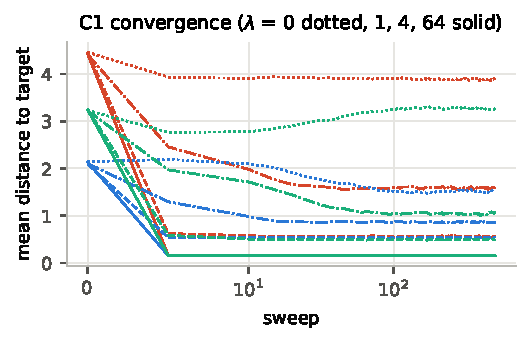
\includegraphics[width=0.48\textwidth]{cond_convergence.pdf}
\caption{C1: mean distance to the target along the chains (colour = target, line style = $\lambda$).}
\end{figure}
